\section{The Polynomial-time Hierarchy}
    \subsection{Basic definitions and properties}
        \begin{frame}{Definitions}
            \begin{block}{Definition: $\Sigma_k^P$}
                $ \Sigma_0^P := P$\\
                For $k\geq 1:$ \\
                $L \in \Sigma_k^P \iff $ there are polynomials $p_1, p_2,..., p_k$ and a polynomial-time predicate $F$ s.t.:
                $$x \in L \leftrightarrow 
                    \existss{y_1 \in S_1\text{ }}{}
                    \foralll{y_2 \in S_2\text{ }}{}
                    \exists ...\underset{y_k \in S_k}{Q} F(x,y_1,...,y_k)$$
                where $S_i := \{0,1\}^{p_i(|x|)}$  
            \end{block}
        \end{frame}
        \begin{frame}{Definitions}
            \begin{block}{Definition: $\Pi_k^P$}
                $ \Pi_0^P := P$\\
                For $k\geq 1:$ \\
                $L \in \Pi_k^P \iff $ there are polynomials $p_1, p_2,..., p_k$ and a polynomial-time predicate $F$ s.t.:
                $$x \in L \leftrightarrow 
                    \foralll{y_1 \in S_1\text{ }}{}
                    \existss{y_2 \in S_2\text{ }}{}
                    \forall ...\underset{y_k \in S_k}{Q} F(x,y_1,...,y_k)$$
                where $S_i := \{0,1\}^{p_i(|x|)}$  
            \end{block}
        \end{frame}

        
        \begin{frame}{Definitions}
            \begin{block}{Definition: The Polynomial-time Hierarchy $PH$}
            $PH := \bigcup_{i \in \mathbb{N}} \Sigma_i^P \cup \Pi_i^P $
            \end{block}
        \end{frame}
    
        \begin{frame}{Structural Properties}  
            for all $i\in \mathbb{N}$: 
            \begin{enumerate}
                \item $\Pi_i^P = co\Sigma_i^P $
                \pause
                \item $\Sigma_i^P \subseteq \Sigma_{i+1}^P \cap \Pi_{i+1}^P$
                \item $\Pi_i^P \subseteq \Sigma_{i+1}^P \cap \Pi_{i+1}^P$
                \pause
                \item (?)$\Sigma_i^P \subset \Sigma_{i+1}^P$
            \end{enumerate}
        \end{frame}

        \begin{frame}{Equivalent definition}
            \begin{block}{lemma}
                For $i\geq 1, L \in  \Sigma_{i+1}^P \iff $there is a polynomial $p$ and $A \in \Pi_i^P$:
                $$x \in L \leftrightarrow \existss{y\in \{0,1\}^{p(|x|)}}{} <x,y> \in A$$
            \end{block}
            \pause
            \begin{block}{Proof}
                $<x,y> \in A \leftrightarrow \foralll{y_1 \in S_1\text{ }}{}
                    \existss{y_2 \in S_2\text{ }}{}
                    \forall ...\underset{y_k \in S_k}{Q} F(<x,y>,y_1,...,y_k)$\\
                for some polynomial F and $S_i := \{0,1\}^{p(|x|)_i}$ for polynomials $p_1,p_2,..., p_k$. Putting this in the equation gives us the desired result.
            \end{block}
        \end{frame}

        \begin{frame}{Collapsibility}
            \begin{block}{lemma}
                For $i\geq 1, L \in  \Pi_{i+1}^P \iff $there is a polynomial $p$ and $A \in \Sigma_i^P$:
                $$x \in L \leftrightarrow \foralll{y\in \{0,1\}^{p(|x|)}}{} <x,y> \in A$$
            \end{block}
            \pause
            \begin{block}{Theorem: PH is collapsible}            
                $i \geq 1 $ \& $ \Pi_i^P = \Sigma_i^P \to PH = \Sigma_i^P$
            \end{block}
        \end{frame}

        \begin{frame}{Collapsibility}
            \begin{proof}
                \small{
                It suffices to show that 
                $i\geq1 \text{ $\&$ } \Sigma_k^P = \Pi_k^P 
                \to \Sigma_k^P = \Sigma_{k+1}^P$:\\
                $L \in \Sigma_{k+1}^P \iff$ there is a polynomial $p$ and $A \in \Pi_i^P$:
                $$x \in L \leftrightarrow \existss{|y|=p(|x|)}{} <x,y> \in A$$
                $\iff$ there are $A \in \Sigma_i^P$ and $p$:
                 $...$\\
                $\iff$ there are $p,p'$ and $B \in \Pi_{i-1}^P$:
                $$x \in L \leftrightarrow \existss{|y|=p(|x|)}{} \existss{|y'|=p'(|x|)}{} <x,y,y'> \in B$$
                $\iff$ there are $p'' = p+p'$ and $B \in \Pi_{i-1}^P$:
                $$x \in L \leftrightarrow \existss{|y''|=p"(|x|)}{} <x,y''> \in B$$
                $\iff L \in \Sigma_k^P$.
                }
            \end{proof}
        \end{frame}
            

        \begin{frame}{Scheme of the Polynomial-time hierarchy}            
            \begin{figure}
                \centering
                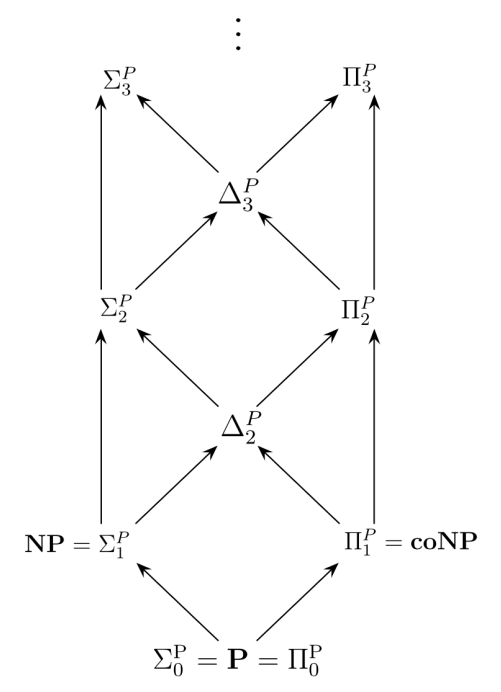
\includegraphics[scale=.4]{images/PH.png}
                \caption{The Polynomial-time Hierarchy.}
                \label{fig:The Polynomial-time Hierarchy}
            \end{figure}
        \end{frame}

    \subsection{Relationships to other  complexity classes}
        \begin{frame}{Relationships to other complexity classes}  
            \begin{block}{Review: NP}
                $L \in NP \iff $ there is a polynomial $p$ and a Polynomial-time predicate $F$ s.t.:
                $$x \in L \iff \existss{y \in O(p(|x|))}{} F(x,y)$$
            \end{block}
        \end{frame}
        \begin{frame}{Relationships to other  complexity classes}
            \begin{block}{Lemma}
                $NP = \Sigma_1^P$
            \end{block}
            \begin{block}{Proof}
                \begin{enumerate}
                    \item $\existss{p}{}  y \in O(p(|x|) \iff \existss{p'}{}  y\leq  \, p'(x)$
                    \item  for one direction use padding to fix the length of y
                    \item for the other direction check the length of y in algorithm
                \end{enumerate}                
            \end{block}
        \end{frame}
        
        \begin{frame}{Relationships to other  complexity classes} 
            \begin{block}{Definition: BPP}
                $L \in BPP \iff $ there is a polynomial $p$ and a polynomial-time randomized algorithm (predicate) $F$ s.t.:
                $$x \in L \implies \underset{r\in \{0,1\}^{p(|x|)}}{Pr}(F(x,r)) \geq 2/3$$
                $$x \notin L \implies \underset{r\in \{0,1\}^{p(|x|)}}{Pr}\ (F(x,r)) \leq 1/3$$
            \end{block}
            \begin{table}
                \centering
                \begin{tabular}{rcc}
                     & $F(x,r)$ & $\neg F(x,r)$ \\\hline
                    $x \in L$ & \(\geq 2/3\) & \(\leq 1/3\) \\
                    $x \notin L$ & \(\leq 1/3\) & \(\geq 2/3\) \\
                \end{tabular}
                \caption{$\underset{r\in \{0,1\}^{p(|x|)}}{Pr}\ (F(x,r))$}
                \label{BPP DEF}
            \end{table}
        \end{frame}
        
        %\begin{frame}{Relationships to other complexity classes}
        %    \begin{lemma}
        %        If $L \in BPP$, then there is a polynomial time algorithm %$A$ such that: $$\underset{r\in \{0,1\}^m} {P}\ (A(x,r) = %right\text{ }answer) \geq 1-\frac{1}{3m}$$
        %        where $m = |x|^k$ for some $k$.
        %    \end{lemma}
        %\end{frame}
        
        %\begin{frame}{Relationships to other complexity classes}
        %    \begin{alertblock}{proof}
        %        There is a polynomial time algorithm A; $\underset{r'\in \%{0,1\}^m} {P}\ (A(x,r') = right\text{ }answer) \geq \frac{2}{3m}$
        %        Design F(x,r):= which takes     
        %    \end{alertblock}
        %\end{frame}

        \begin{frame}{Relationships to other complexity classes}
            \begin{block}{lemma}
                $BPP$ is closed under complement.
            \end{block}
            
            \begin{block}{Fact}
                $BPP \subseteq \Sigma_2$
            \end{block}
        \end{frame}
                
        \begin{frame}{Relationships to other complexity classes}
            \begin{block}{Sipser–Lautemann theorem}
                $BPP \subseteq \Sigma_2^P \cap \Pi_2^P$
            \end{block}
        \end{frame}
        
        \begin{frame}{Relationships to other  complexity classes}
            \begin{block}{Theorem}
                $PH \subseteq PSPACE$
            \end{block}
        \end{frame}

        \begin{frame}{Relationships to other  complexity classes}
            \begin{block}{Proof}
                It is sufficient to show that for any $i$ if $\Pi_i \in PSPACE$ then $\Sigma_{i+1} \in PSPACE$:\\
                Suppose $L \in \Sigma_{i+1}$ then there is a polynomial $p$ and $A \in \Pi_i^P$:
                $$x \in L \leftrightarrow \existss{y\in \{0,1\}^{p(|x|)}}{} <x,y> \in A$$
                $A$ is decidable in $PSPACE$ by hypothesis, thus $\existss{y\in \{0,1\}^{p(|x|)}}{} <x,y> \in A$ is decidable in $PSPACE$ using an odometer.
            \end{block}
        \end{frame}

        \begin{frame}{Relationships to other  complexity classes}
            \begin{block}{Lemma}
                For all $i$: $\Sigma_i^P$  is closed under $\leq_p$
            \end{block}
            \pause
            \begin{block}{Proof}
                $A \leq_p B \iff$ there is a polynomial algorithm $R$:
                    $$x\in A \iff R(x) \in B$$
                Now suppose $B \in \Sigma_i^P$ then:
                $$x \in A \leftrightarrow 
                    \existss{y_1 \in S_1\text{ }}{}
                    \foralll{y_2 \in S_2\text{ }}{}
                    \exists ...\underset{y_k \in S_k}{Q} F(R(x),y_1,...,y_k)$$
                where $S_i := \{0,1\}^{p_i(|R(x)|)}$
            \end{block}
        \end{frame}
        \begin{frame}{Relationships to other  complexity classes}
            \begin{block}{Theorem}
                $PH = PSPACE \implies PH$ Collapses.
            \end{block}
            \pause
            \begin{block}{proof}
                $PH = PSPACE \implies PH$ have a complete problem which is in $\Sigma_i$ for some $i$ and since $\Sigma_i$ is closed under $\leq_p$: $\Sigma_i = PH$
            \end{block}
        \end{frame}
        
        \begin{frame}{Relationships to other  complexity classes}   
            \begin{enumerate}
                \item $NP = \Sigma_1^P $ $\&$ $ CoNP = \Pi_1^P$
                \pause
                \item $P = NP \iff P = PH$
                \pause
                \item $BPP \subseteq \Sigma_2^P \cap \Pi_2^P $
                \pause
                \item $PH \subseteq PSPACE$
                \pause
                \item $PH = PSPACE \implies PH$ Collapses.
            \end{enumerate}
        \end{frame}
        
        \begin{frame}{Complexity classes}            
            \begin{figure}
                \centering
                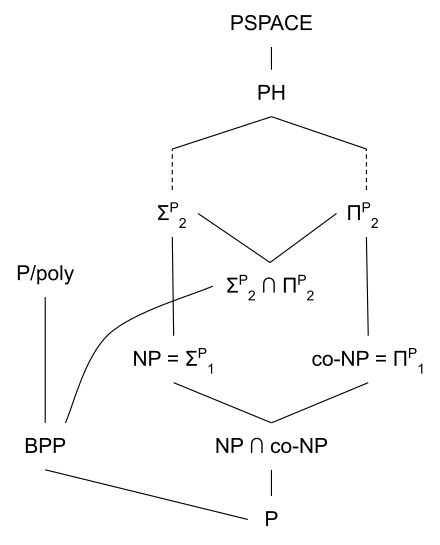
\includegraphics[scale=0.5]{images/PH2.png}
                \caption{Complexity Classes Inclusion Tree}
                \label{fig:focuslogo}
            \end{figure}
        \end{frame}